\documentclass[14pt]{extarticle}
\usepackage[T1]{fontenc}
\usepackage[utf8]{inputenc}
\usepackage{amsmath,amssymb}
\usepackage[russian]{babel}
\usepackage{graphicx}

\begin{document}
\title{\text{Требования к воспроизведению текстовой}\\ \text{информации на экране}}
\maketitle

\section{Введение}

Чтение утомляет глаза и может испортить зрение, поэтому для книг, а в особенности для учебников, давно существуют гигиенические стандарты, которые определяют размер и рисунок шрифта, расстояние между строками, яркость букв и белизну страниц. Иногда по тем же правилам оформляют электронные учебники. Это решение, принятое, безусловно, из благих побуждений, на самом деле ошибочно, потому что наше зрение при чтении с экрана испытывает совсем иные нагрузки, нежели при чтении с листа.

Чтение с экрана требует повышенной концентрации внимания и интенсивной умственной деятельности. Человеческий глаз приспособлен рассматривать предметы в отраженном свете, и наблюдение светящегося объекта противоречит самой его природе.

Одним из самых главных недостатков чтения с экрана является то, что разрешение на мониторе значительно ниже, чем у текста, напечатанного на бумаге. Из-за этого буквы кажутся несколько неровными. А также исключительно негативную роль, как с точки зрения производительности, так и осознания и запоминания информации играет мигание и дрожание строк текста.

Эти и некоторые другие особенности делают чтение с экрана дисплея довольно утомительным занятием. Поэтому для электронного текста должны быть свои гигиенические стандарты, определяющие оптимальные размеры текстовых блоков, интервалы между строками и словами, выбор удобочитаемого шрифта и цветовых решений, соответствующих особенностям восприятия человека. Эти и другие аспекты оформления текстовой информации на экране будут рассмотрены в данной работе.

\section{Характеристики восприятия информации}

Деятельность человека, сидящего перед экраном монитора, начинается с приема информации: в его сознании отражаются свойства воспринимаемого с экрана объекта и формируется его перцептивный (чувственный) образ. Физиологической основой формирования перцептивного образа является работа зрительного анализатора. Существует определенный набор условий, обеспечивающих нормальную работу зрительного анализатора:

\begin{enumerate}
	\item яркость объекта должна лежать в определенных пределах (надежное различие цветовых оттенков возникает при яркости 175~Кд*м$^2$);
	\item контрастность изображения относительно фона должна выбираться с учетом размеров объекта: чем меньше его размер, тем выше должна быть его контрастность;
	\item следует учитывать, что наибольшую чувствительность глаз имеет к излучению желто-зеленого цвета, наименьшую - к фиолетовому и красному;
	\item размер символа должен быть согласован с остротой зрения человека; нужно также учитывать, что он влияет на скорость и правильность восприятия информации;
	\item все поле зрения, охватываемое глазом, можно разбить на три зоны: центрального зрения, где наиболее четко различаются детали; ясного видения, где можно опознать объект без мелких деталей; периферического зрения, где предметы обнаруживаются, но не распознаются;
	\item зрительное ощущение нарастает и спадает постепенно, в сумме это время составляет 0.5 секунды (при резком действии прерывистого раздражителя возникает ощущение мельканий, которые при определенной частоте сливаются в ровный немигающий свет~---~оптимальная частота сигнала в случае миганий~---~3*10 Гц).

\end{enumerate}

Чтобы работа с компьютером была удобной, пользователь при взаимодействии с ней должен ощущать комфорт.

\begin{table}[h]
\resizebox{\textwidth}{!}{%
\begin{tabular}{|l|l|l|}
\hline
\textbf{Факторы}           & \textbf{Вызываются}                           & \textbf{Влияют на}    \\ \hline
Социальные факторы         & Психологическим климатом                      & Эмоциональный комфорт \\ \hline
Физическая эргономика      & Аппаратным обеспечением                       & Физический комфорт    \\ \hline
Психологическая эргономика & Качеством разработки программного обеспечения & Умственный комфорт    \\ \hline
\end{tabular}%
}
\end{table}

\section{Текст}

\subsection{Плотность и размеры текстовой информации}

Количество информации, отображаемой на экране, называется экранной плотностью. Исследования показали, что, чем меньше экранная плотность, тем отображаемая информация наиболее доступна и понятна для пользователя и наоборот, если экранная плотность большая, это может вызвать затруднения в усвоении информации и ее ясном понимании.

Существует мнение , что необходимо оставлять пустым приблизительно половину экрана. На то, что большинство пользователей Интернет предпочитают беглое ознакомление внимательному чтению, во многом влияет именно качество современных мониторов. Чтение с экрана оказывает повышенную нагрузку на зрение и приблизительно на 25\% медленнее, чем чтение текста с бумаги. Поэтому не удивительно, что люди пытаются свести к минимуму объем читаемой информации.

Для правильного выбора разреженности строк, также измеряемой в пунктах, необходимо учитывать размер используемого шрифта. В современных издательских системах разреженность строк определяется автоматически на уровне 120\% от выбранного размера шрифта. В то время как в ГОСТ Р ИСО 9241-3-2003 о требованиях к визуальному отображению информации на дисплее гласит, что минимальный интервал между строками текста должен равняться одному пикселю. Однако это правило не подразумевает оптимальную величину интервала. В HTML-учебниках принято отмечать, что межстрочный интервал в тексте должен быть больше кегля (размер шрифта); как правило, он составляет не менее 115\% кегля. Такая пропорция основана на необходимости дополнительного места для диакритических знаков, имеющихся во многих европейских языках. Межстрочный интервал выбирается и из эстетических соображений: текст читать легче, если между строчками есть пустое пространство.

Также к плотности расположения текста на экране относятся интервалы межсимвольные и между словами. Для шрифтов, не имеющих концевых засечек, интервал между знаками должен быть не менее ширины одного пикселя. Для знаков с засечками интервал между засечками соседних знаков не должен быть меньше одного пикселя. Минимальный интервал между словами должен быть не менее ширины одного знака (для соразмерных шрифтов следует использовать заглавную букву <<N>>).

Чтобы вычислить оптимальную величину текстового поля необходимо вывести зависимость размера отображаемой информации от угла обзора человека и его удаленности от экрана монитора.

Человек имеет следующие характеристики зрения по области охвата: область наилучшего видения 1.5 градуса; зона ясного видения 15 градусов; максимальная зона видения 35 градусов.

Дисплей должен находится от глаз оператора на расстоянии 600-700 мм, в соответствии с инструкцией по охране труда для оператора ЭВМ.

Подставляя в формулу описанные выше входные данные, получаем, что ширина текста при чтении с монитора не должна превышать 20 см. Ширина строки (колонки) определяется количеством знаков, которые могут быть на ней помещены. Обычно оптимальным считается расположение в одной строке от 45 до 60 символов. Стоит обратить внимание на наличие связи между шириной строки и размером выбранного шрифта: чем меньше размер шрифта, тем короче строка. Иными словами, меньший размер шрифта дает возможность поместить больше символов на заданной площади листа. Иначе глазные мышцы будут совершать много лишних движений и поэтому уставать намного быстрее.

\subsection{Верстка текста}

Верстка~---~термин, родившийся в эпоху ручного набора текста, он относится к изготовлению печатной формы, состоящей из гранок набранного текста. При электронном наборе версткой называется компоновка, размещение текста на площади оригинал-макета, который предназначен для последующего воспроизведения и тиражирования средствами печати.

Гармоничность и пропорциональность - главные условия высококачественной верстки текста. Фрагменты текста должны располагаться на экране так, чтобы взгляд пользователя перемещался по экрану в привычном направлении.

При электронном наборе возможно несколько вариантов выравнивания текста: по левому или правому краю, относительно центральной линии (центрирование) и блочное выравнивание (на ширину полосы). В полиграфии подобное редактирование носит название выключки строк. Оно предполагает равномерное увеличение или уменьшение пробелов между словами (а иногда и между буквами) для доведения строки до заданного формата.

В эпоху ручного набора для выключки строк приходилось изменять толщину шпации~---~строчного пробельного материала между словами. При электронном наборе любой текст также может быть "выключен", но при этом его строки будут автоматически выравниваться вдоль условной вертикальной линии, которая может располагаться слева, справа или в центре. Кроме того, текст может иметь полную выключку, когда строки выравниваются с обеих сторон.

Набор с выключкой влево используется для любых длинных текстов, особенно при узкой полосе набора. Считается, что текст, выровненный по левому краю, читать удобнее всего, т.к. он соответствует направлению чтения слева направо(в русском языке, как и в большинстве других европейских языков, принят порядок чтения слева направо). Выключка вправо придает набранному тексту оригинальность и рекомендуется в тех случаях, когда, например, подпись к рисунку должна находиться справа от него и заканчиваться у края картинки. Набор с выключкой по центру используется для заголовков и ввода стихотворного текста. Ввод текста с выключкой по формату хорошо известен по книгам.

Наиболее популярным типом верстки HTML страниц на сегодняшний момент является табличная верстка (верстка в колонки). На самых известных новостных сайтах мы видим, что текст разбит на колонки. Причем одна из них отводиться для основного текста, а другая для так называемых "приманок". <<Приманкой>>~---~называется краткая аннотация статьи. Второе применение малой колонки сводиться к становлению навигации сайта. Там также могут располагаться ссылки, новости и баннеры.

Важным элементом компоновки текста является его корректное размещение на площади экранной формы. Особенно это касается оформления названий и заголовков. Несоразмерно высокое, как и слишком низкое расположение названия или заголовка выглядит некрасиво. Казалось бы, самое простое~---~разместить строки в центральной части формы. Располагая текст в центре, нужно быть осторожным. Давно известно, что из-за оптического обмана средняя линия страницы или формы кажется несколько ниже реальной середины листа. Чтобы преодолеть этот эффект, следует размещать строку немного выше средней линии, тогда будет казаться, что она расположена как раз посередине экранной формы.

Разместить одну строку на экранной форме несложно. Ситуация существенно усложняется, когда приходится размещать целый блок или несколько блоков текста. Подобная компоновка будет выглядеть гармоничной только в том случае, если учесть <<весовое соотношение>> блоков. Блоки, расположенные над оптической средней линией, обязательно должны уравновешиваются блоками, размещенными под ней.

Под весом понимается величина, зависящая от размера шрифта и плотности печати текста. При одинаковом весе двух компонуемых блоков их следует размещать на одинаковом расстоянии от оптической средней линии. Если же вес блоков различен, то для сбалансированного размещения "более тяжелый" блок текста следует придвинуть ближе к средней линии.

Ширина полей, окружающих текст, также немаловажный фактор, который должен учитываться при верстке. Оставленные вокруг текста поля, значительно облегчают чтение: наличие широких полей – основной принцип хорошей читаемости. Текст не должен находиться у самого края экрана, к тому же длинные строки сложно читать. Однако, слишком широкие поля (больше 1/3 экрана) не улучшают читаемость. Не существует конкретных рекомендаций в числовом эквиваленте по поводу ширины этих полей~---~известно, что они должны гармонично и симметрично располагаться вокруг текстовых сегментов, габариты которых были вычислены ранее в данной работе.

Также, при формировании информации на экране следует помнить.

\begin{itemize}
	\item При очень плотном расположении строк, изображение на экране будет выглядеть слишком темным. Этого следует по возможности избегать, регулируя плотность строк межстрочными интервалами.
	\item Содержимое полей в таблицах должно не <<прижиматься>> к краю экрана, а располагаться около горизонтальных или вертикальных осей.
	\item Меню, содержащее относительно небольшой объем информации, должно быть смещено в левую верхнюю часть экрана (плюсы расположения меню сверху проявляется не только в известном следствии закона Фиттса, заключающемся в том, что в таким образом расположенное меню бесконечно проще попасть мышкой (мышка упирается в край экрана), но и в том, что оно позволяет делать окна намного более лёгкими и простыми на вид без ущерба для функциональности - все необходимые функции можно оставить в меню, а в окне оставить только самое важное, основное содержимое).
	\item Один и тот же тип информации должен появляться всегда в одном и том же месте экрана, пользователю должен быть предоставлен максимально удобный интерфейс и он должен быть освобожден от необходимости трудоемкого поиска необходимой ему информации.
	\item Верхние две или три строки экрана обычно резервируются для вывода заголовка и состояния системы. Заголовок показывает, в каком месте системы находится пользователь; область состояния показывает пункты меню верхнего уровня и служит для вывода подтверждений о том, что система работоспособна.

\end{itemize}

\subsection{Размер шрифта}

Правильный выбор необходимого шрифта, его размера, цвета и написания очень сильно влияет, во-первых, на эффективность всего дизайна интерфейса в целом, во-вторых, на удобство чтения.

Шрифт~---~гарнитура определенного кегля и начертания.

Кегль~---~размер гарнитуры подобранный для данного шрифта. Измеряется в пунктах.

Начертание~---~стиль написания гарнитуры. Например~---~полужирный, италик (наклонный) или одновременно и то и другое.

Гарнитура~---~совокупность литер (символов), объединенных одним стилем и общей идеей.

Различимость шрифтовых знаков ухудшается из-за низкого разрешения экрана ПК. Разрешение~---~величина, определяющая количество точек (пикселей) на единицу площади (или единицу длины). Поэтому, если эта величина мала, при сравнимо больших размерах дисплея, то, соответственно, экранный шрифт должен быть крупнее, чем при печати на бумаге, а именно~---~соответствовать как минимум типографскому кеглю цицеро, равному 14 пунктам. Важно помнить, что размер шрифта должен быть таким, чтобы его было легко читать. У некоторых пользователей могут быть проблемы со зрением, поэтому шрифт лучше всего делать масштабируемым (шрифт, размер которого может быть изменен пользователем).

\subsection{Гарнитура шрифта}

Выбранная гарнитура шрифта должна вписываться по своему виду и стилю в общий дизайн интерфейса, и должен быть хорошо виден и читаем для пользователей. Существует огромное количество самых различных шрифтов. У каждого отдельного шрифта есть своё название, причём многие из них существуют в различных вариантах основного вида и рисунка. Шрифт должен привлечь внимание читателя и помочь ему сосредоточиться на чтении текста, выделить наиболее важные аргументы. Также следует помнить различную психологическую нагрузку, которую несут различные гарнитуры.

\begin{itemize}
	\item Шрифты с засечками сочетают мужскую авторитарность с органичным, гуманистическим стилем, более притягательным для женщин. Различные исследования показали, что шрифты с засечками читаются легче на бумаге, так как засечки помогают взгляду передвигаться от буквы к букве, и буквы при этом не сливаются друг с другом.
	\item Шрифты без засечек обладают малым эмоциональным зарядом и ассоциируются с практичностью и здравомыслием. Они являются надежным выбором для тех, кто жаждет гармонии и не озабочен самовыражением посредством шрифтового оформления.
	\item Гарнитурные шрифты с большими круглыми буквами <<О>> и <<хвостиками>> воспринимаются как дружественные и <<человечные>>, возможно потому, что их начертание подражает образу человеческого лица.
	\item Прямолинейные и угловатые шрифты ассоциируются с непреклонностью, жестокостью; они характеризуются холодностью, безликостью и механистичностью. В терминах психоанализа их определяют такие выражения, как "эмоционально зажатый".
	\item Шрифты рукописного стиля~---~это попытка передать дружелюбие и близкие отношения. В свое время эти шрифты использовались банками, желающими избежать ощущения <<казенности>> путем имитации в письмах <<персональной подписи>>. Используя рукописные стили, крупные корпорации ставят задачу казаться более дружелюбными, <<близкими к народу>>.
	\item Декоративные шрифты чаще всего их используют, чтобы подчеркнуть новизну, яркость, индивидуальность. Но, лучше никогда не использовать их в качестве основного текста: они являются неудобочитаемыми, а так же при этом пропадает их эффектность.
\end{itemize}

Для отображения основного текста обычно используют шрифт небольшого размера.

Такой текст воспринимается значительно лучше, если используются рубленые шрифты, например, Arial, Verdana, а не шрифты с засечками (например, Times New Roman). Это происходит от того, что современные мониторы имеют сравнительно низкую разрешающую способность, и поэтому для того, чтобы четко отобразить засечки шрифта размером 10 пунктов попросту не хватает пикселов. С другой стороны, большинство людей предпочитает читать на бумаге текст, набранный именно шрифтами с засечками (в подавляющим большинстве книг используется именно такие шрифты).

Поэтому мы оказываемся перед лицом своеобразного парадокса. Возможно, этот парадокс разрешится сам собой, когда мониторы будут улучшены настолько, чтобы чтение с экрана стало бы таким же быстрым и приятным, как чтение книги.

Как показывает практика экранной типографии, в основном пользователи используют такие гарнитуры, как Times New Roman (Образец), Verdana (Образец), Arial (Образец), изначально имеющиеся в памяти любого ПК. Рассмотрим особенности этих гарнитур.

Шрифт Verdana~---~самый популярный шрифт, применяемый при верстке web-сайтов. Он выделяется гигиеническими и художественными достоинствами. Он рассчитан на воспроизведение с низким разрешением, прост по рисунку, его пропорции удобны и красивы. Шрифт выглядит легким, открытым и без труда воспринимается с дисплея.

Шрифт Arial похож на предыдущий, также не менее популярен, но чуть мельче и уже. Также имеет хорошую читабельность, если только не использовать его маленьких размеров.

Times New Roman~---~хороший шрифт с засечками оптимизированный для вывода текстов на экран. Очень распространённый и поэтому установлен и применяется по умолчанию во всех редакторах. Times New Roman хорошо подходит для web-документов, предназначенных для последующей печати.

Можно использовать и какой либо из красивых и эффектных декоративных шрифтов, но с ними надо быть осторожными и не забывать о чувстве меры, дабы не повлиять на удобочитаемость, выводимого на экран, текста.

Считается, что использование в текстах не более двух~---~трёх разных шрифтов на одной страничке или форме является наиболее комфортным условием для восприятия информации пользователем.

\subsection{Начертание шрифта}

Каждый тип шрифта имеет несколько начертаний символов, например, полужирный, курсив, полужирный курсив, обычный. Кроме того, можно ввести подчеркивание символов и фрагментов текста.

Полужирный текст~---~очень хороший прием, однако использовать его надо умеренно. Следует выделять полужирным начертанием лишь отдельные слова и никогда~---~фразы. Также не стоит и перебарщивать: при большом количестве полужирных слов web-страница становится слишком пестрой.

Такое начертание, как италик (курсив) создает эффект цитатного текста. При умелом использовании курсива можно добиться большей близости с пользователем~---~текст с цитированием всегда внушает больше доверия, чем простой текст.

Следующий способ выделения текста не связан с начертаниями, но от этого его эффективность не страдает. Этот метод основан на смене цвета выделяемого текста. Однако, при чрезмерном использовании смены цвета web-страница или программная форма может либо запестрить, как в случае с полужирным начертанием, так и свести на нет непосредственную роль смены цвета, то есть выделенный текст перестанет обращать на себя внимание.

Одним из самых малоэффективных способов привлечения внимания к тексту считается~---~подчеркивание. Подчеркивание ассоциируется с http-ссылкой. Пользователь может вас неправильно понять и начать бегать мышкой по подчеркиваниям от слова к слову. Это утомляет и, как следствие портит общее впечатление от сайта или программного средства. Ко всему прочему линия подчеркивания проходит через нижние выносные части литер и снижает читабельность текста.

Ну и самый неэффективный прием~---~перечеркивание. Он также как и предыдущий прием, сильно портит удобочитаемость текста, кроме того, область его применения не ясна. Предположительно, он может быть использован для представления текстовых сегментов, которые принадлежали первоначальной версии текста, но позднее были удалены.

\subsection{Регистр букв}

Заглавная буква в тексте (начало предложения), прописная буква, идущая после заглавной~---~это как раз и есть различный регистр букв. Проще можно было бы сказать размер букв, но это будет не совсем верно. Размер прописной буквы может составить 50 пикселей, а заглавная буква может иметь меньший размер, но оставаться при этом заглавной. Регистр это разница в написании одного и того же символа, разное представление одних и тех же буквенных знаков.

Текст в нижнем регистре читается приблизительно на 13\% быстрее, чем текст, который напечатан полностью в верхнем регистре. Символы верхнего регистра наиболее эффективны для информации, которая должна привлечь внимание, но частое использование этого способа приводит к перегрузке интерфейса.

\subsection{Динамическое отображение текста}

Неудобство при чтении может вызвать текст, оформленный в виде <<бегущей строки>>, а также мигающий и переливающийся текст. Но злоупотреблять использованием данных эффектов не стоит, хотя иногда они могут быть вполне оправданными:

\begin{itemize}
	\item бегущая строка зачастую используется для отображения информации большого объема на маленьких дисплеях, таких, как на телефонах или других портативных устройствах;
	\item движение, мигание или изменение позиции текста это очень эффективный метод выделения информации, поскольку глаз имеет специальный детектор для движущихся элементов.
\end{itemize}

Человеческий глаз воспринимает не отдельные буквы, а группы букв или слов. Это свойство глаза, охватывать группы букв, их форму, а также определённую длину строк является фактором, ускоряющим или замедляющим чтение, а также из него следует, что всплывающая строка воспринимается легче и комфортней бегущей. Однако использование и выпадающей строки может вызывать раздражение у человека-оператора, ведь время экспозиции отображения текста в такой строке не может быть для каждого разным. Для одного человека строка будет перелистываться чересчур медленно, а другой не успеет прочитать отображаемую информацию.

Таким образом, можно сделать вывод, что динамического отображения текста стоит избегать, кроме тех случаев, когда необходимо привлечь внимание пользователя, отвлечь его от основного содержимого окна приложения.

\section{Особенности выбора цвета}

\subsection{Цветовое восприятие человека}

Цвет~---~мощный визуальный инструмент, его необходимо использовать очень осторожно, чтобы не вызвать дискомфорта у пользователя ошибочными цветовыми комбинациями.

То, что мы видим на экране монитора, является всего лишь комбинацией трех цветов: Red (красный), Green (зеленый) и Blue (синий). Задача дизайнера~---~сочетать их так, чтобы работать с разрабатываемым программным средством было максимально комфортно.

Многочисленные исследования наиболее комфортных сочетаний цветов при выводе данных на экран дисплея, выявили ряд параметров для оценки качества отображения. Одним из основных является четкость восприятия цветовых образов.

\begin{figure}[ht]
    \centering
    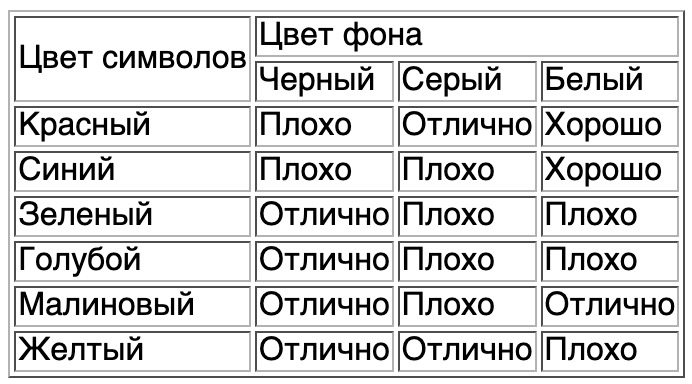
\includegraphics[width=0.5\textwidth]{assets/1.jpeg}
\end{figure}

Вплоть до последнего времени считалось, что белый фон малоэффективен по сравнению с другими цветами. Однако с появлением высококачественных дисплеев, имеющих высокое разрешение, выяснилось, что работоспособность оператора, считывающего черные буквы на белом фоне, на треть выше, чем на цветном фоне.

\begin{figure}[ht]
    \centering
    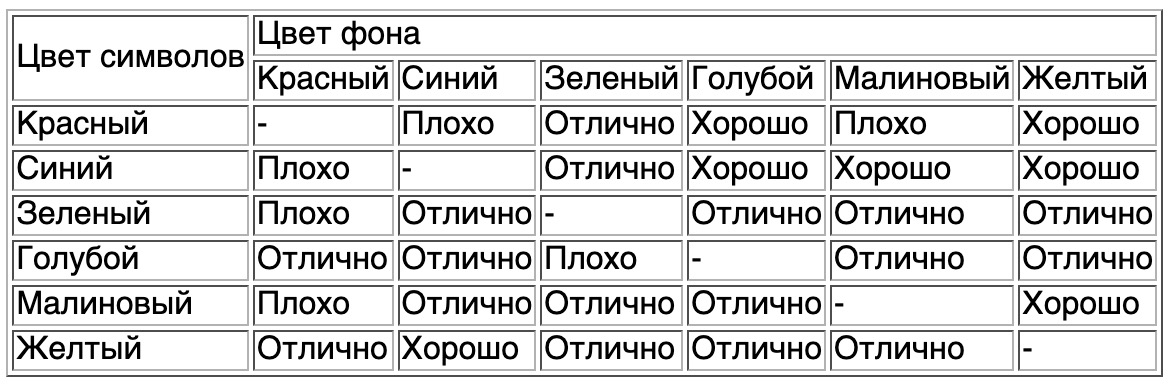
\includegraphics[width=0.5\textwidth]{assets/2.jpeg}
\end{figure}

Однако текст на белом фоне~---~это стандартный, но не самый лучший вариант, поскольку сильный контраст цветов влечет дополнительную утомляемость. Избежать этого можно простым подбором цветовой пары текст - фон.

\begin{figure}[ht]
    \centering
    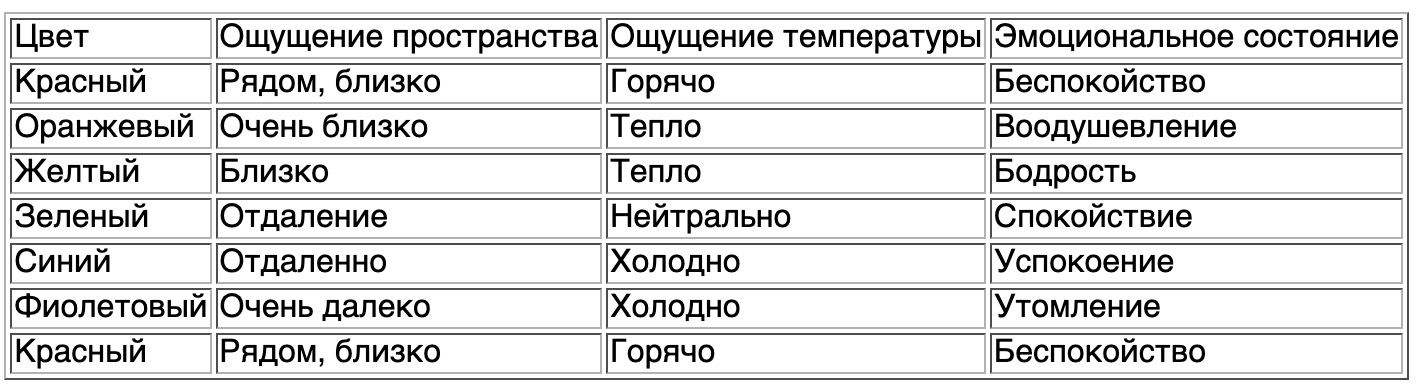
\includegraphics[width=0.5\textwidth]{assets/3.jpeg}
\end{figure}

Для цвета основного текста лучше подходит универсальный черный, хотя возможны и варианты (темно-коричневый, темно-синий и т. д.). Для фона следует использовать мягкие пастельные тона, причем лучший визуальный эффект дает не сплошная заливка фона выбранным цветом, а мягкий расфокусированный текстурный фон.

В пределах одного тематического раздела цвет и текстура фона должны оставаться постоянными для всех страниц.

\subsection{Принцип функционального соответствия}

Наиболее активными для привлечения внимания считаются красный и синий цвета, далее желтый, зеленый и белый. Поэтому красный и синий рекомендуется использовать для кодирования наиболее важных объектов. Синий цвет из-за его тенденции к размытости границ малопригоден для окраски мелких графических элементов, требующих предельной четкости изображения. Его чаще применяют в качестве акцентирующей подложки под выделяемые графические элементы. Там, где требуется хорошая видимость деталей изображения, безошибочная и быстрая их идентификация, применяют желто-зеленые, желтые и оранжевые цвета, обеспечивающие наиболее четкую фокусировку изображения на сетчатку глаза.

Важно помнить, что люди связывают с различными цветами особые представления: красный цвет~---~цвет опасности, зеленый~---~нормы и т. д.

\subsection{Принцип физиологического соответствия}

Цвета по яркости и контрастности не должны выходить за пределы, вызывающие утомление зрения. Пониженная светимость изображения вызывает перенапряжение мышц хрусталика глаза и, как следствие, снижение остроты зрения. Повышенная яркость (более 175 кд*м$^2$) приводит к снижению цветовой чувствительности.

Следует, по возможности, отказаться от использования яркостных контрастов как признака кодирования, заменяя их контрастами по цветности, более комфортными для зрителя. Желательно использовать в одном изображении сочетание взаимно дополнительных цветов так, чтобы соблюдался принцип цветового баланса (близость общего тона гаммы к серому).

\subsection{Принцип эмоционального соответствия}

Цвета должны вызывать эмоциональную реакцию, улучшающую самочувствие и повышающую работоспособность человека. Стимулирующим фактором является сбалансированное сочетание в цветовой гамме теплых и холодных цветов. Теплые цвета, как наиболее выступающие и предметные, привлекают и удерживают внимание, холодные, используемые чаще как фоновые, оказывают компенсирующее воздействие, обеспечивая поддержание цветовой чувствительности на высоком уровне.

С точки зрения эмоциональной привлекательности, в цветовой палитре экранных кадров не следует использовать: подавляющий и угнетающий темно-фиолетовый, холодный темно-зеленый, яркий лимонно-желтый и зелено-желтый, бледно-розовый и некоторые другие оттенки и сочетания, вызывающие негативные реакции.

\subsection{Рекомендации по использованию цвета при формировании оконного интерфейса}

Существует определенное количественное соотношение между изображением и фоном (<<равновесие>> фигуры и фона), характеризующее оптимальную для восприятия величину изображения~---~его масштаб масштаб не должен быть, с одной стороны, слишком мелким, чтобы объект не терялся в отведенном ему поле экрана, а с другой~---~чересчур крупным, чтобы не возникало ощущение <<тесноты>> на экране. Также, величина оптимального масштаба зависит от выбранной цветовой гаммы: изображение, построенное на насыщенных цветах, резко контрастирующих по яркости с фоном, <<требует>> меньшего размера, чем изображение с нюансными отношениями по яркости и насыщенности.

При отображении на экране дисплея текстовой информации хорошие результаты получаются для следующих сочетаний цвета символов и фона: белый на черном, зеленый на черном, желтый на черном, желтый на синем. Наихудшие результаты по скорости чтения и восприятию данных получаются при выводе красных символов на синем фоне, синих на черном, красных на черном.

Фоновые изображения не должны влиять на удобочитаемость текста. Некоторые фоновые изображения, даже привлекательные сами по себе, затрудняют чтение наложенного на них текста. Фоновый рисунок должен оставаться на заднем плане, и чем он скромнее, тем лучше. При длительной работе с объектами на разноцветном фоне наступает так называемая <<цветовая усталость>> глаз, которая приводит к общему утомлению даже в том случае, если выбраны комфортные сочетания цветов. Поэтому для поддержания положительного эмоционального состояния цветовую палитру экрана считается, что надо периодически менять, используя три-четыре <<рабочих>> варианта цветовых сочетаний.

По статистике, около 10\% мужчин и 1\% женщин обладают той или иной степенью дальтонизма, поэтому нельзя использовать для контрастной окраски фона и текста красный и зеленый цвета~---~люди имеющие эту особенность зрения не видят разницы между этими цветами. Не следует использовать более четырех цветов на одной экранной форме. Чем больше цветов, тем больше шанс, что дизайн будет рябить в глазах. Профессионалы используют много цветов только в том случае, если целевая аудитория~---~дети (чтобы не скучали) или домохозяйки (чтобы заметили товар на полке). Также во избежание развития состояния усталости рекомендуется также включать в сценарий графического диалога специальные реабилитационные кадры вставки. В качестве <<разгрузочных>> изображений могут использоваться, например, цветовые мозаичные структуры с эффектом интерференции, рассчитанные на неполное пространственное смешение цветов (цепочки ярких, контрастных цветовых точек). Такие структуры способствуют быстрому восстановлению цветовой чувствительности.

\section{Выводы}

В электронных изданиях, в отличие от печатных, следует использовать преимущественно короткие четкие предложения и сжатые параграфы, позволяя пользователю предельно быстро просмотреть экран в поисках нужной информации.

Большинство специалистов считают, что познавательная ценность электронного текста измеряется тремя характеристиками: первоначальная реакция пользователя на текст, привлекательность текста, его ясность. Если пользователю неприятен стиль оформления текста, то его производительность при работе с ним, конечно, снизится. Поэтому при форматировании текста для электронных изданий необходимо учитывать особенности восприятия информации человеком с экрана дисплея.

Существуют требования к отображению текста на экране, основанные не только на эстетических соображениях и особенностях зрительного анализатора человека, но и на конкретных свойствах дисплея компьютера: на его разрешающей способности, частоте мерцания, угле обзора и т.д.

\end{document}